\documentclass[main.tex]{subfiles}
\begin{document}

\section{Compare and contrast I2C \textit{(Inter-Integrated Circuit)} and SPI \textit{(Serial Peripheral Interface)}.} \label{section:compare_i2c_spi} 
% Note this question is meant to give more details on these two protocols that are initially introduced as a part of signalling.tex which is intended to be a much broader question.

\spoilerline

\subsection{I2C}
I2C is a \textit{half-duplex} (can either transmit or receive, but not both simultaneously) digital protocol developed by Phillips in 1982 \cite{sparkfun_i2c_history}. It enables a host device\footnote{I2C does support multiple master devices, however, this article focuses on the significantly more prevalent single-master implementation.} (referred to as a \textit{master}\footnote{The phrases 'master' and 'slave' are slowly being phased out due to their origins. However, at time of writing, 'master' and 'slave' are the most commonly used terms and are used in this guide. Alternative verbiage includes 'controller' for master and 'peripheral' or 'target' for slave.}) to communicate with multiple peripheral devices (referred to as \textit{slaves}) over a two-wire serial bus. 
% Unfortunately at the time of writing, master/slave is the pervasive industry standard terms.

\subsubsection{Physical Layer}
The physical layer of I2C consists of two wires: SDA (Serial Data) and SCL (Serial Clock). By definition, it is a \textit{synchronous} protocol, meaning that the clock signal is shared between the master and slave devices. The SDA line carries the data, while the SCL line carries the clock signal. The SDA line is bidirectional, allowing both the master and slave to transmit and receive data. The SCL line is unidirectional, controlled by the master device (though it can be asserted by a slave to pause communications to give time for processing, known as \textit{clock stretching}). A hardware bus diagram is shown in Figure \ref{fig:i2c_bus}.

\begin{figure}[H]
    \centering
    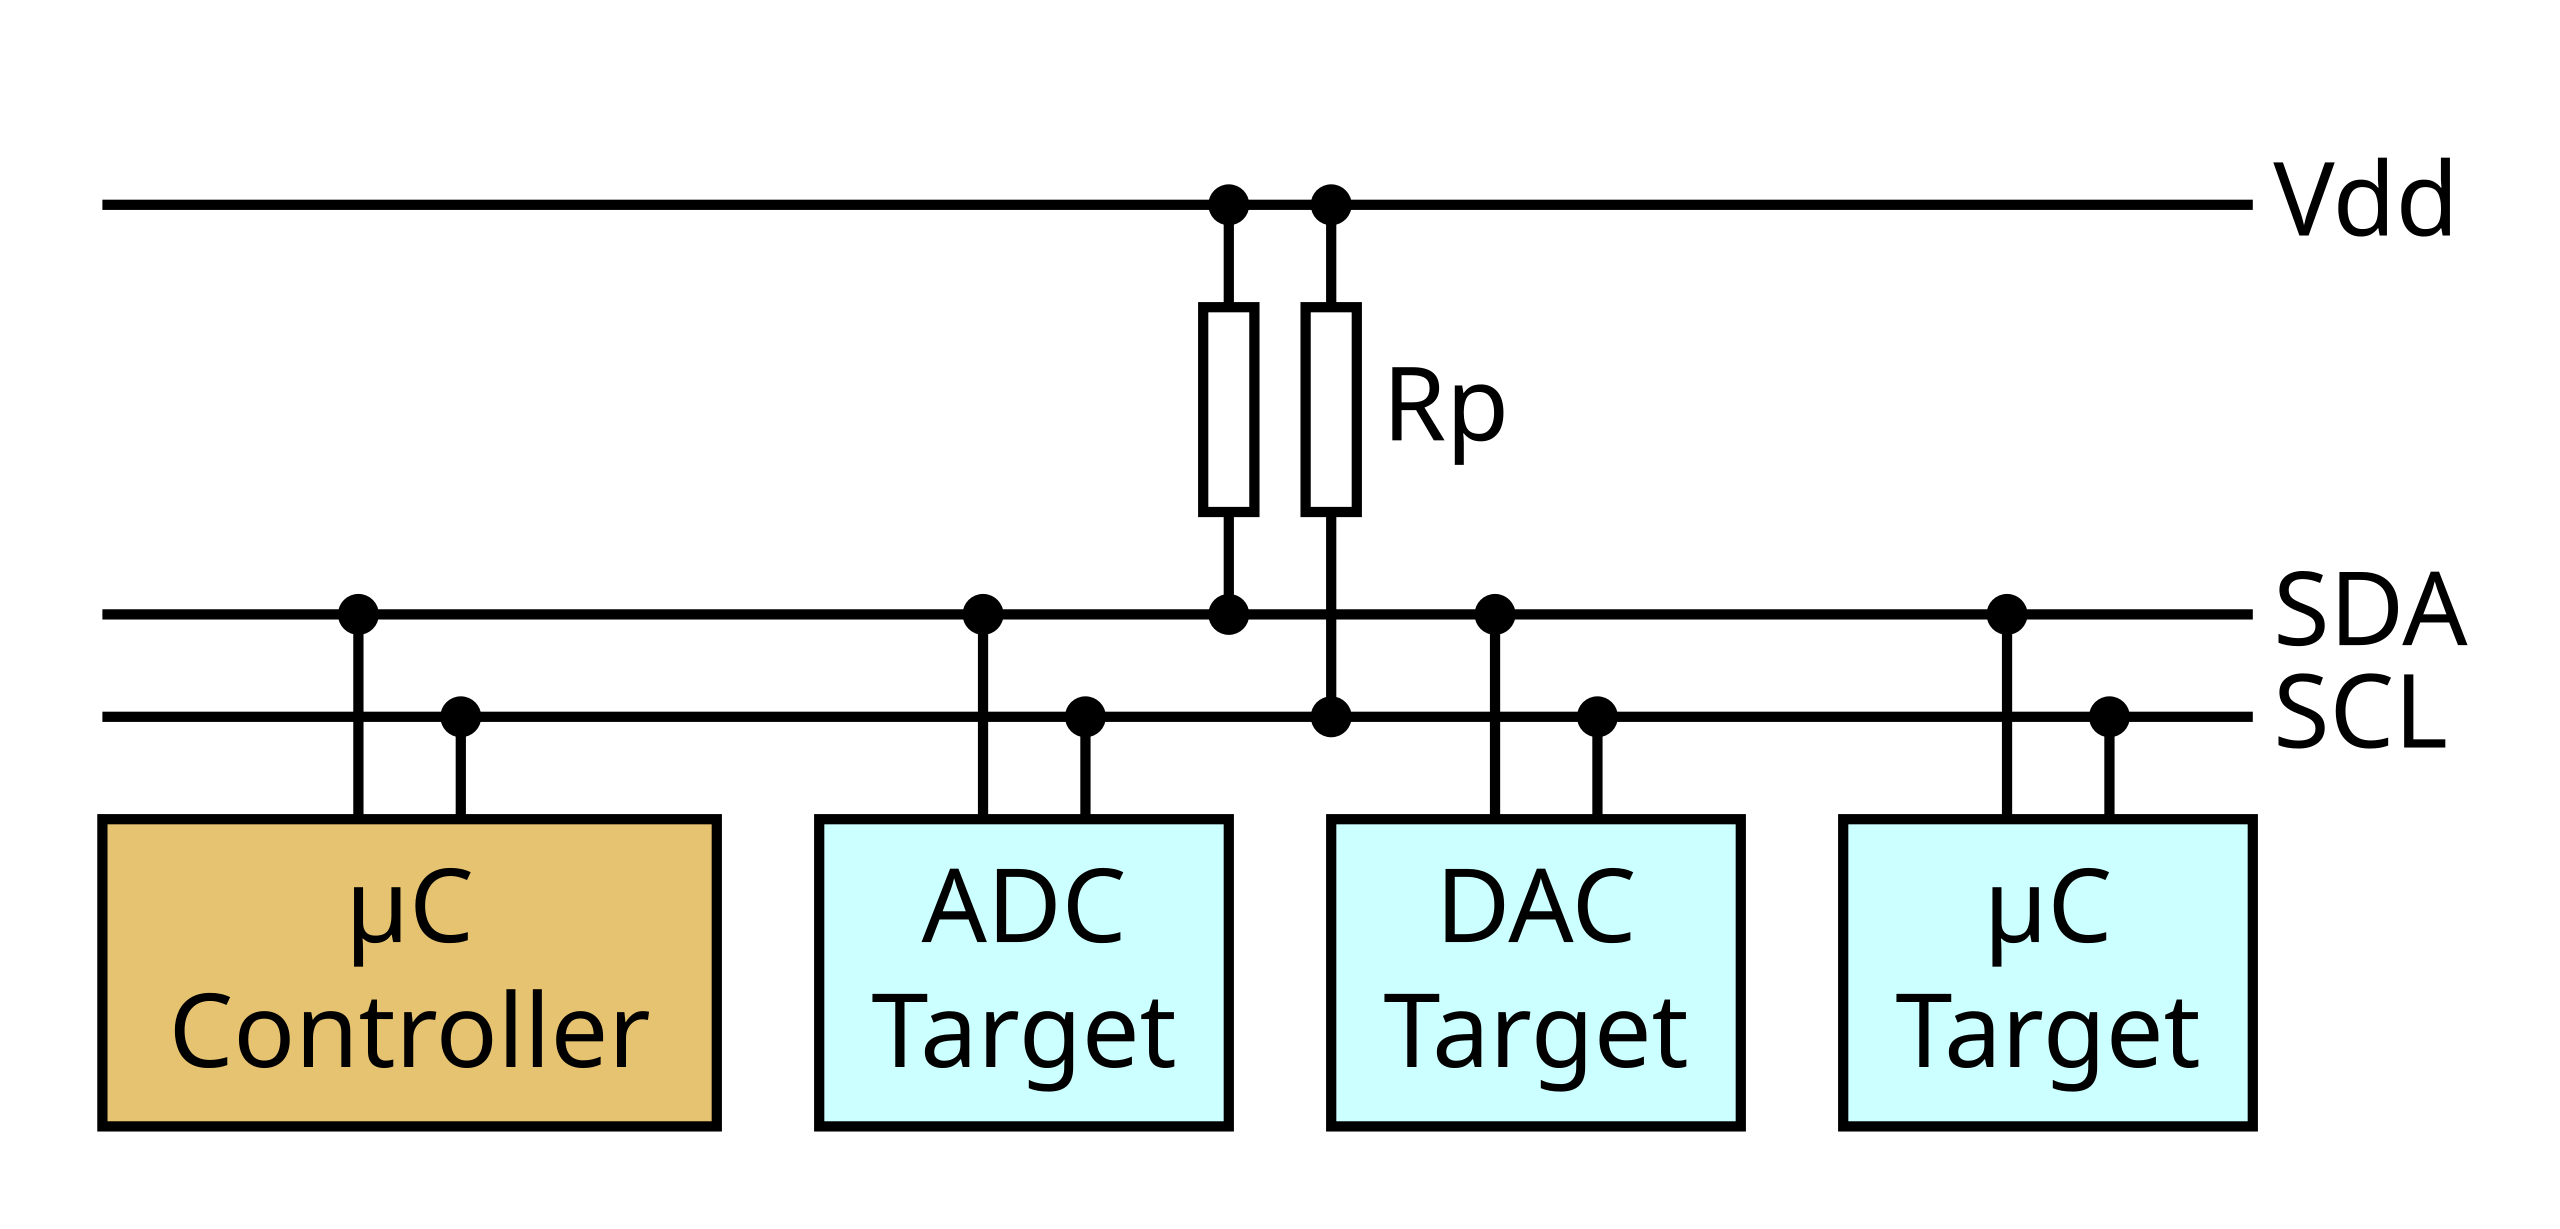
\includegraphics[scale=0.09]{images/I2C_controller-target.png}
    \caption{I2C Bus Diagram, Source: Wikipedia \cite{wikipedia_i2c_bus_image}}
    \label{fig:i2c_bus}
\end{figure}

\noindent The bidirectional nature of the SDA and SCL lines is achieved by using \textit{open-drain} drivers. Open-drain drivers can pull the line low, but not drive it high, instead relying on a \textit{pull-up} resistor to "pull the voltage up". This is contrast to a \textit{push-pull} driver, which can drive the line both high and low. Open-drain drivers, while advantageous in ensuring that the bus can never be shorted by two devices driving the line with different voltages, suffers from slower rise/fall times due to the pull-up resistor forming an RC circuit with the parasitic bus capacitance, and limits the maximum bus speed to 400kHz traditionally, though higher speeds just above 1 MHz are permissible in newer versions of the specification.
% More information about RC circuit diagram is not given here as it will be covered in "passive_circuits.tex"

\subsubsection{Data Format}
The data format of I2C features the following components, and is shown graphically in Figure \ref{fig:i2c_data_format}:
\begin{enumerate}
    \item \textbf{Start Condition}: The master device initiates communication by pulling the SDA line low while the SCL line is high, signalling the beginning of a transfer.
    \item \textbf{Address (7 bits)}: A 7-bit address is transmitted on the SDA line to indicate which slave device the master wishes to communicate with.
    \item \textbf{Read/Write Bit}: The 8th bit of the address byte is used to indicate whether the master wishes to read from or write to the slave device. A \texttt{0} indicates a write operation, while a \texttt{1} indicates a read operation. If a read is requested, control of the SDA line is transferred to the slave device.
    \item \textbf{Acknowledge Bit}: After each byte is transmitted, the receiving device (master or slave) sends an acknowledge bit. If the receiving device pulls the SDA line low, it indicates that it has received the byte and is ready for the next byte. If the SDA line remains high, it indicates that the receiving device is not ready, or that an error occurred.
    \item \textbf{Data Byte(s)}: Data bytes are transmitted in 8-bit chunks, with each byte followed by an acknowledge bit.
    \item \textbf{Stop Condition}: The master device signals the end of the transfer by, in the case of a write, releasing the SDA line while the SCL line is high, or in the case of a read, sending a \texttt{NACK} (Not Acknowledge) bit followed by a stop condition.
\end{enumerate}

\begin{figure}[H]
    \centering
    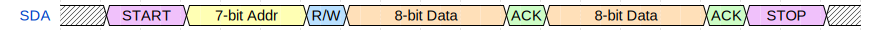
\includegraphics[scale=0.4]{generated_images/svg_generated/i2c_data_format.png}
    \caption{2 Byte I2C Data Frame Format}
    \label{fig:i2c_data_format}
\end{figure}

\subsection{SPI}
SPI was developed by Motorola \cite{SPI_history} and is a \textit{full-duplex} (simultaneous transmit and receive) synchronous serial communication protocol. It is commonly used in embedded systems to communicate between a master device and one or more slave devices. SPI is a \textit{four-wire} protocol, consisting of the following signals: MISO (Master In Slave Out), MOSI (Master Out Slave In), SCLK, and CS (Chip Select). A timing diagram of a 1-byte SPI transaction is shown in Figure \ref{fig:spi_timing}.

\begin{figure}[H]
    \centering
    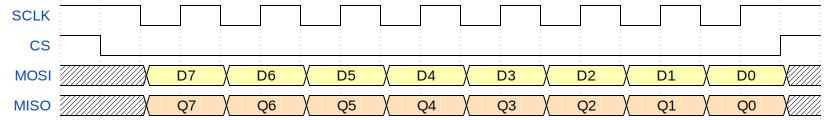
\includegraphics[scale=0.4]{generated_images/svg_generated/spi_waveform.png}
    \caption{1-byte SPI Timing Diagram}
    \label{fig:spi_timing}
\end{figure}

\noindent Unlike I2C, SPI does not have a standard addressing scheme, and the master device must \textit{assert} (pull down) a CS line to connected to the slave device it wishes to communicate with - the requirement for each slave device to feature its own CS line increases SPI's wiring complexity. Owing to the push-pull nature of SPI drivers, the bus is faster than I2C (low MHz range). The bus diagram is shown in Figure \ref{fig:spi_bus} (Note the diagram in Figure \ref{fig:spi_bus} uses \textit{SS} for \textit{Slave Select}, which is synonymous with \textit{CS}).

\begin{figure}[H]
    \centering
    \includegraphics[scale=0.2]{generated_images/svg_generated/SPI_three_slaves.png}
    \caption{SPI Bus Diagram, Source: Wikipedia \cite{wikipedia_SPI_bus}}
    \label{fig:spi_bus}
\end{figure}

\subsection{Comparison}
\begin{itemize}
    \item \textbf{Bus Speed}: SPI is faster than I2C, with speeds in the MHz range (ex: 1-40 MHz) compared to I2C's 400 kHz range due to the differences in drive type. As a result, SPI is often used in applications where the transfer speed is required to be high.
    \item \textbf{Wiring Complexity}: I2C requires, at most, two wires, regardless of the number of devices on the bus owing to its addressing scheme. A SPI master requires at least four wires, plus an additional wire for each slave device (each slave will require 4 wires).
    \item \textbf{Frame Format}: I2C has a more complex frame format than SPI, with start and stop conditions, address bytes, and acknowledge bits, which can assist in debugging unresponsive slave devices. However, SPI has a simpler frame format, with no addressing scheme and no acknowledge bits, which reduces the overhead of each transaction and affords more flexibility in the data format.
    % Comparison of I2C and SPI with analog signals is further elaborated on in signalling.tex
\end{itemize}

\subsection{Follow-ups}
\begin{itemize}
    \item What are strategies for dealing with conflicting I2C addresses?
    \item What are strategies for dealing with the possibly-large number of CS lines in SPI?
    \item How are pull-up resistance values selected for I2C?
\end{itemize}

\end{document}
